\documentclass{article}
\usepackage[margin=0.75in]{geometry}
\usepackage{graphicx} % Required for inserting images
\usepackage{tikz}
\usetikzlibrary{positioning}
\usepackage{amsfonts} % For mathcal
\usepackage{amsmath} % For align* environment

% Define TikZ styles
\tikzstyle{latent} = [circle, draw, minimum size=1cm]
\tikzstyle{obs} = [rectangle, draw, minimum size=1cm]

% Define edge command
\newcommand{\edge}[2]{\draw[->] (#1) -- (#2);}

\title{Quick HMM note}
\author{Justin Chiu}
\date{September 2025}

\begin{document}

\maketitle

\section{Motivation}
Worked on scaling out classical probabilistic language models in the past.
Looks kind of like state-space models, but discrete states.
Trained the largest HMM ever.
We can go much bigger now.

\section{Hidden Markov Models}

For times $t$, model states $z_t$, and tokens $x_t$,

\begin{center}
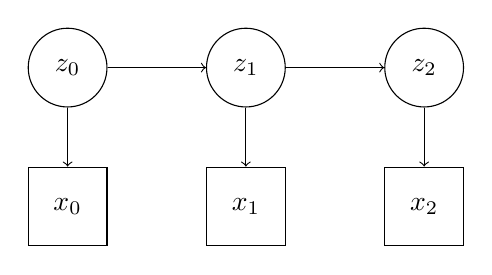
\begin{tikzpicture}[]
\node[latent] (z0) {$z_0$} ;
\node[latent] (z1) [right=1.25cm of z0] {$z_1$} ;
\node[latent] (z2) [right=1.25cm of z1] {$z_2$} ;

\node[obs]    (x0) [below = 0.75cm of z0] {$x_0$};
\node[obs]    (x1) [below = 0.75cm of z1] {$x_1$};
\node[obs]    (x2) [below = 0.75cm of z2] {$x_2$};

\edge {z0} {x0};
\edge {z1} {x1};
\edge {z2} {x2};
\edge {z0} {z1};
\edge {z1} {z2};
\end{tikzpicture}
\end{center}

\section{Joint distribution and parameterization}
$$p(x,z) = \prod_t p(x_t \mid z_t)p(z_t \mid z_{t-1})$$
with
\begin{align*}
\textnormal{start state } & p(z_1),\\
\textnormal{transitions } & p(z_t \mid z_{t-1}),\\
\textnormal{and emissions } &  p(x_t \mid z_t)
\end{align*}

Abstraction: Generate these parameters using neural network. Code can focus only on these three inputs.
Also abstract away training code (nanogpt-style).

Show training loop and torch module code.

\section{Inference: Forward algorithm (joint)}
We can recursively compute the joint probability
$p(x_t,z_t, x_{<t})$ for each $t$.

Base case: $p(z_1)$.

Inductive hypothesis: we have previous joint $p(z_{t-1}, x_{<t})$.

By total probability:
$$p(x_t, z_t,  x_{<t}) = p(x_t \mid z_t)\sum_{z_{t-1}} p(z_t \mid z_{t-1}) p(z_{t-1}, x_{<t}).$$

The joint probability is simple to implement, but not numerically stable.
Log-space for avoiding underflow, summing very small numbers.

Just a sequence of matrix-vector products
$$
\pi_t = o_t \odot (A^\top\pi_{t-1}),
$$
where
\begin{align*}
\textnormal{previous joint } & \pi_{t-1} \in [0,1]^Z: \pi_{t-1}[z_{t-1}] = p(z_{t-1}, x_{<t}),\\
\textnormal{transition matrix } & A \in [0,1]^{Z\times Z}: A[z_{t-1},z_{t}] = p(z_t \mid z_{t-1}),\\
\textnormal{and emission vector } &  o_t \in [0,1]^Z: o_t[z_t] = p(x_t \mid z_t).
\end{align*}

Zoom in on evidence\_loop.

\section{Inference: Forward algorithm (bmm)}
Log-space operations is too slow, since the operaitons not fused.
Change implementation to use bmm for matmul when possible.
Key is to avoid underflow during summations.

Inductive hypothesis: previous state posterior $p(z_{t-1} \mid x_{<t})$.
Need need state prior, observation evidence, and state posterior.
\begin{align}
p(z_t \mid x_{<t}) &= \sum_{z_{t-1}} p(z_t \mid z_{t-1}) p(z_{t-1} \mid x_{<t}) \\
p(x_t \mid x_{<t}) &= \sum_{z_t} p(x_t \mid z_t)p(z_t \mid x_{<t}) \\
p(z_t \mid x_t, x_{<t}) &= \frac{p(x_t \mid z_t) p(z_t \mid x_{<t})}{p(x_t \mid x_{<t})}.
\end{align}

We do (1) in probability space but (2) in log-space.
(1) is well-conditioned for small enough $Z$ because (3) ensures it through normalization.
It's ok for 32k states. 64k was not ok.

Zoom in on evidence\_loopbmm.

\section{Advanced: Low-rank bmm and emission sparsity}
You can speed things up even further with other tricks.

Trick 1: If you make the transition matrix low-rank, you can just do two small matmuls instead of a big one.
This turns $O(Z^2)$ into $O(ZR)$ with $2R < Z$.

Trick 2: Emission sparsity (words can only be emit in certain states) reduces computation quite a lot.
It limits the effective state size at any given time.
This improves both speed and numerical stability.

\begin{center}
\resizebox{0.8\width}{0.8\height}{
\input{trellis_no_drop.tex}
}
\end{center}

\end{document}

